\subsubsection{Cloud Service}

Der Cloud Service wurde wie im Konzept beschrieben umgesetzt.
Er dient dazu die Konfiguration des Praxisrufsystems persistent zu verwalten und Benachrichtigungen von Mobile CLients entgegenzunehmen und gemäss Konfiguration über den angebundenen Message Service an andere Mobile Clients zu weiterzuleiten.

Um diese Aufgaben zu erfüllen, bietet der Cloud Service eine REST API unter www.praxisruf.ch/api an.
Diese API ist unter www.praxisruf.ch/api erreichbar und über Baisic Authentication geschützt.

Zu Test- und Entwicklungszwecken ist die API zudem über www.praxisruf.ch/swagger-ui.html erreichbar.
Das Swagger Interface dokumentiert die API die der Cloud Service anbietet.
Dies Beinhaltet die verfügbaren Endpunkte und das Model welches für Input und Ouput Werte dieser API dienen.

\begin{figure}[h]
    \begin{minipage}[b]{1\textwidth}
        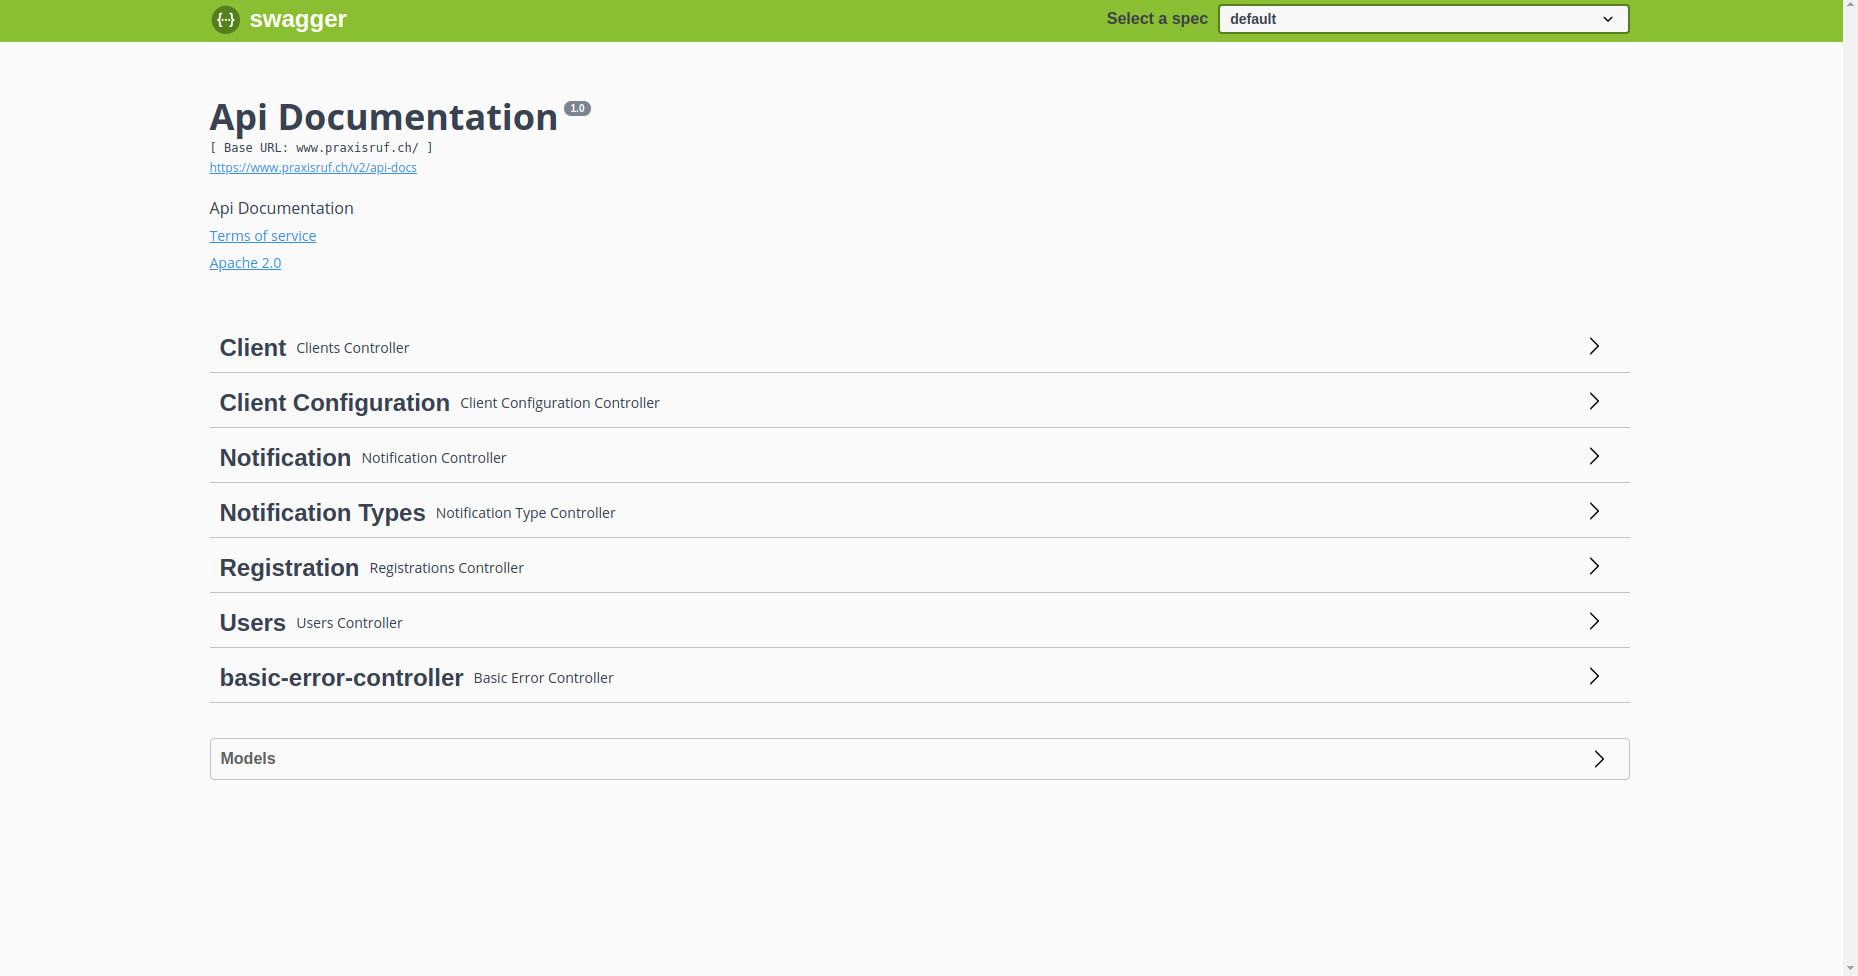
\includegraphics[width=\textwidth]{graphics/screenshots/cloud/swagger-home}
        \caption{Swagger UI}
    \end{minipage}
    \label{fig:swagger}
\end{figure}
\clearpage
